\documentclass[10pt]{article}
\usepackage[margin=1in]{geometry}

\usepackage{biblatex}
\addbibresource{./references.bib}

\usepackage{hyperref}
\usepackage{xcolor}
\hypersetup{
    colorlinks,
    linkcolor={red!70!black},
    citecolor={blue!70!black},
    urlcolor={blue!90!black}
}

\usepackage{tikz}
\usetikzlibrary{shapes,arrows}
\usetikzlibrary{arrows.meta}

\begin{document}
This is an overview of the material point method.
While there are many variants due to the experimental nature of MPM, this document is focused on the current implementation.
For a more general review, please see the paper by \textcite{buzzi08}.

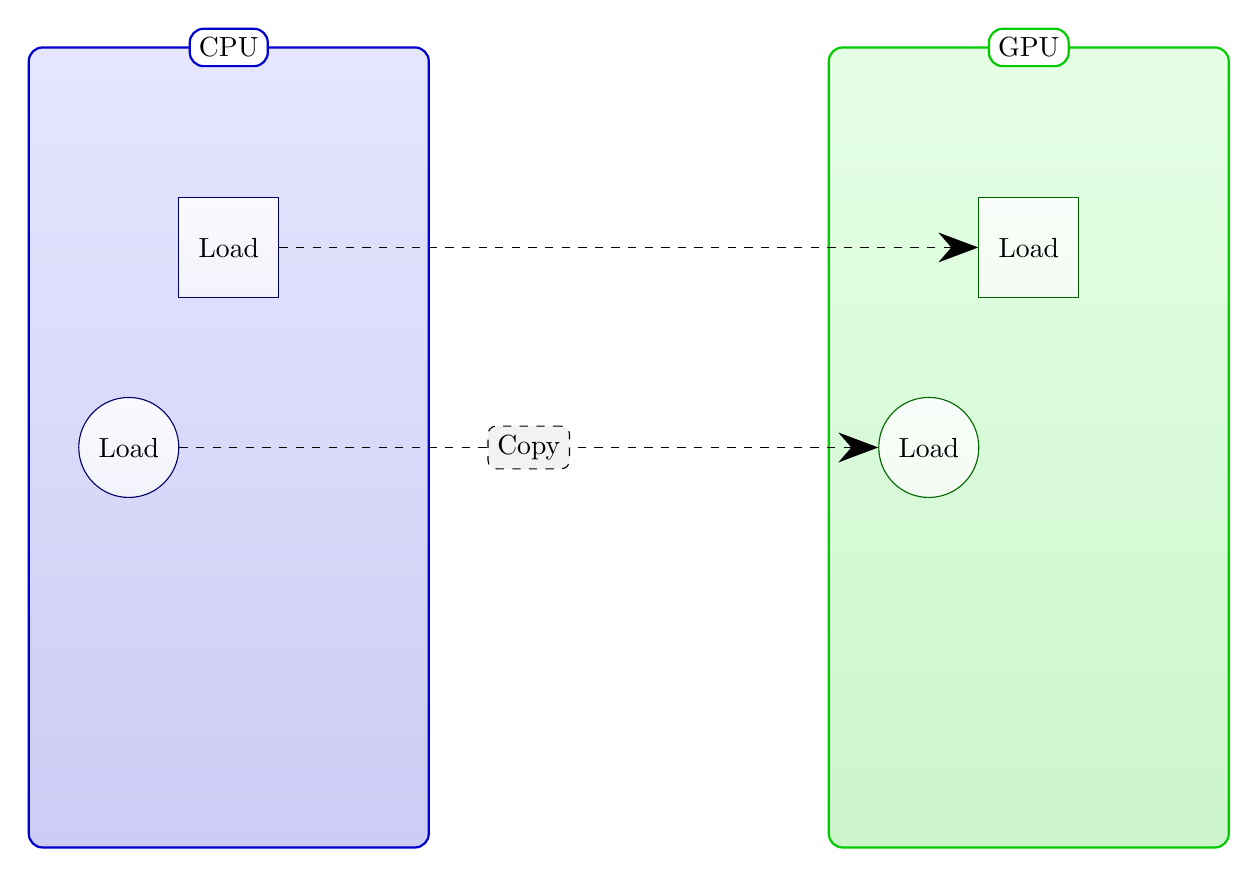
\begin{tikzpicture}
\tikzstyle{gpuborder}=[thick, draw=green!80!black]
\tikzstyle{gpushade}=[shade, top color=green!10, bottom color=green!80!black!20]
\tikzstyle{ongpu}=[draw=green!40!black, shade, top color=green!70!black!2, bottom color=green!70!black!5]
\tikzstyle{cpuborder}=[thick, draw=blue!80!black]
\tikzstyle{cpushade}=[shade, top color=blue!10, bottom color=blue!80!black!20]
\tikzstyle{oncpu}=[draw=blue!40!black, shade, top color=blue!70!black!2, bottom color=blue!70!black!5]
\tikzstyle{copy}=[draw=black,dashed,-{Stealth[scale=3]}]
\tikzstyle{function}=[draw=black,dotted,-{Stealth[scale=3]}]
\tikzstyle{functionbox}=[rounded corners=3pt, draw=black, fill=black!5]
\tikzstyle{ms}=[minimum size=0.5in]

% Background 'containers'
\path[cpushade, cpuborder, rounded corners=5pt] (0, 0) -- (0, 4in) -- (2in, 4in) node[pos=0.5, fill=white, cpuborder] {CPU} -- (2in, 0) -- cycle;
\path[gpushade, gpuborder, rounded corners=5pt] (4in, 0) -- (4in, 4in) -- (6in, 4in) node[pos=0.5, fill=white, gpuborder] {GPU} -- (6in, 0) -- cycle;

\node[oncpu, ms, circle] (init-pstate) at (0.5in, 2in) {Load};
\node[oncpu, ms] (init-mstate) at (1in, 3in) {Load};

\node[ongpu, ms, circle] (gpu-init-pstate) at (4.5in, 2in) {Load};
\node[ongpu, ms] (gpu-init-mstate) at (5in, 3in) {Load};

\path[copy] (init-pstate) -- (gpu-init-pstate) node[functionbox, pos=0.5] {Copy};
\path[copy] (init-mstate) -- (gpu-init-mstate);
\end{tikzpicture}

\printbibliography

\end{document}
